%%
%% This is file `sample-sigplan.tex',
%% generated with the docstrip utility.
%%
%% The original source files were:
%%
%% samples.dtx  (with options: `all,proceedings,bibtex,sigplan')
%% 
%% IMPORTANT NOTICE:
%% 
%% For the copyright see the source file.
%% 
%% Any modified versions of this file must be renamed
%% with new filenames distinct from sample-sigplan.tex.
%% 
%% For distribution of the original source see the terms
%% for copying and modification in the file samples.dtx.
%% 
%% This generated file may be distributed as long as the
%% original source files, as listed above, are part of the
%% same distribution. (The sources need not necessarily be
%% in the same archive or directory.)
%%
%%
%% Commands for TeXCount
%TC:macro \cite [option:text,text]
%TC:macro \citep [option:text,text]
%TC:macro \citet [option:text,text]
%TC:envir table 0 1
%TC:envir table* 0 1
%TC:envir tabular [ignore] word
%TC:envir displaymath 0 word
%TC:envir math 0 word
%TC:envir comment 0 0
%%
%%
%% The first command in your LaTeX source must be the \documentclass
%% command.
%%
%% For submission and review of your manuscript please change the
%% command to \documentclass[manuscript, screen, review]{acmart}.
%%
%% When submitting camera ready or to TAPS, please change the command
%% to \documentclass[sigconf]{acmart} or whichever template is required
%% for your publication.
%%
%%


\documentclass[sigplan, anonymous=false]{acmart}
\usepackage{colortbl}

\makeatletter
\renewcommand{\subsubsection}{\@startsection{subsubsection}{3}{0pt}%
  {0\baselineskip \@plus 2\p@ \@minus .2\p@}%
  {.25\baselineskip}%
  {\normalfont\normalsize\bfseries}}
\makeatother

\acmISBN{}
\acmDOI{}
\acmYear{}
\setcopyright{none}
\acmConference{Proceedings of the 24th Winona Computer Science Undergraduate Research Seminar}{April 23, 2024}{Winona, MN, US}
\settopmatter{printacmref=false}
\pagenumbering{gobble}


\usepackage{graphicx} % For including graphics
\usepackage{tabularx} % For creating tables with adjustable column width
\usepackage{multirow} % For multirow cells in tables

%%
%% \BibTeX command to typeset BibTeX logo in the docs
%\AtBeginDocument{%
%  \providecommand\BibTeX{{%
%    Bib\TeX}}}

%% Rights management information.  This information is sent to you
%% when you complete the rights form.  These commands have SAMPLE
%% values in them; it is your responsibility as an author to replace
%% the commands and values with those provided to you when you
%% complete the rights form.
%\setcopyright{acmlicensed}
%\copyrightyear{2018}
%\acmYear{2018}
%\acmDOI{XXXXXXX.XXXXXXX}

%% These commands are for a PROCEEDINGS abstract or paper.
% \acmConference[Conference acronym 'XX]{Make sure to enter the correct
%  conference title from your rights confirmation emai}{June 03--05,
%  2018}{Woodstock, NY}
%%
%%  Uncomment \acmBooktitle if the title of the proceedings is different
%%  from ``Proceedings of ...''!
%%
%%\acmBooktitle{Woodstock '18: ACM Symposium on Neural Gaze Detection,
%%  June 03--05, 2018, Woodstock, NY}
% \acmISBN{978-1-4503-XXXX-X/18/06}


%%
%% Submission ID.
%% Use this when submitting an article to a sponsored event. You'll
%% receive a unique submission ID from the organizers
%% of the event, and this ID should be used as the parameter to this command.
%%\acmSubmissionID{123-A56-BU3}

%%
%% For managing citations, it is recommended to use bibliography
%% files in BibTeX format.
%%
%% You can then either use BibTeX with the ACM-Reference-Format style,
%% or BibLaTeX with the acmnumeric or acmauthoryear sytles, that include
%% support for advanced citation of software artefact from the
%% biblatex-software package, also separately available on CTAN.
%%
%% Look at the sample-*-biblatex.tex files for templates showcasing
%% the biblatex styles.
%%

%%
%% The majority of ACM publications use numbered citations and
%% references.  The command \citestyle{authoryear} switches to the
%% "author year" style.
%%
%% If you are preparing content for an event
%% sponsored by ACM SIGGRAPH, you must use the "author year" style of
%% citations and references.
%% Uncommenting
%% the next command will enable that style.
%%\citestyle{acmauthoryear}
\begin{abstract}
 The QWERTY layout, first developed in the 1870s for typewriters, is the most widely used keyboard layout today despite its inefficiencies. The development of an alternative layout faces two major challenges: quantifying the impact of ergonomic features and effectively navigating the vast search space of possible keyboard layouts. To address these challenges, this paper proposes a data-driven approach using simulated annealing with an objective function derived from empirical typing data. The two data sets used are the 136M Keystrokes data set from Aalto University, containing 8,228 hours of typing data from 168,000 participants, for a controlled analysis of four layouts (AZERTY, Dvorak, QWERTY, and QWERTZ), and the iWeb corpus, one of the largest collections of English text, for frequency analysis. A custom implementation of simulated annealing is employed, featuring a dynamic initial temperature and termination criterion that enables compatibility with different subsets of keys, corpora, and optimization criteria. An analysis reveals a number of factors that impact typing speed. Based on this analysis, a cost function is devised and fine-tuned using the Levenberg-Marquardt algorithm (MAE:$12$ms, R$^2$:$0.78$ at $80$ WPM). To estimate the typing efficiency of a candidate layout, the cost function evaluates the predicted typing time for each sequence in the corpus based on the given layout. The sum of these predicted times serves as the objective function for optimization via simulated annealing. The result is a layout estimated to be $6\%$ faster for typing English compared to QWERTY.
\end{abstract}
% While prior researchers have identified various ergonomic principles, they often rely on observations and theoretical models to inform layout design, rather than developing evaluation models based on quantifiable data.

% Simulated annealing optimizes on estimated typing time for the corpus.

%  

%  like character sequence frequency, finger dexterity, and ergonomic challenges posed by certain positional relationships between keys
%%
%% end of the preamble, start of the body of the document source.
\begin{document}

%%
%% The "title" command has an optional parameter,
%% allowing the author to define a "short title" to be used in page headers.
\title[]{A Data-Driven Approach to Keyboard Optimization}

%%
%% The "author" command and its associated commands are used to define
%% the authors and their affiliations.
%% Of note is the shared affiliation of the first two authors, and the
%% "authornote" and "authornotemark" commands
%% used to denote shared contribution to the research.
%\author{Ben Trovato}
%\authornote{Both authors contributed equally to this research.}
%\email{trovato@corporation.com}
%\orcid{1234-5678-9012}
%\author{G.K.M. Tobin}
%\authornotemark[1]
%\email{webmaster@marysville-ohio.com}
%\affiliation{%
%  \institution{Institute for Clarity in Documentation}
%  \city{Dublin}
%  \state{Ohio}
%  \country{USA}
%}

\author{David Sommerfield}
\email{davidsommerfield.zg@gmail.com}
\affiliation{%
  \institution{Winona State University}
  \department{Computer Science Department}
  \city{Winona}
  \state{Minnesota}
  \country{USA}
}

\maketitle
\pagestyle{plain}



\section{Introduction}
% maybe rewrite, with the invention of the typewriter, yada yada
% The creation of text input methods tailored to English trace back to the era of typewriters. 
QWERTY is a keyboard layout first created for typewriters by Christopher Sholes in the early 1870s \citep{yasuoka2011prehistory}. Today, 150 years since its invention, QWERTY is the most common keyboard layout and, by extension, the most common means of human-computer interaction, extending even to mobile devices. However, what was innovative then has become a source of concern in the modern era, as the design of QWERTY, conceived with little regard for ergonomics, has been linked to user discomfort and repetitive strain injuries \citep{amell2000cumulative}.
% and was further developed and popularized with the success of the Remington No. 2 typewriter, which featured the layout

One of the earliest and most influential advocates for alternative keyboard layouts was August Dvorak, who, along with his collaborator William Dealey, championed a more scientific approach to keyboard design. Their methodology involved motion studies, analysis of high-frequency letters and letter combinations, and a deep understanding of hand physiology, culminating in the creation of the Dvorak Simplified Keyboard in 1932 \citep{hiraga}. Dvorak's efforts in the 1930s marked a significant shift toward a more scientific approach to keyboard design and, at the very least, planted the idea that a more efficient alternative to the QWERTY layout was possible.

Despite these early endeavors, the field has continued to struggle to quantify the precise impact of ergonomic factors on typing efficiency and user comfort. This has led to a continued reliance on theoretical models informed by qualitative observations rather than empirical models derived from robust quantitative data. From these observations, several standard practices have emerged, such as minimizing the distance between keys, arranging columns based on perceived finger dexterity, limiting the use of the same finger twice in succession, and considering character frequency \citep{light1993typewriter}. % For example, \citet{light1993typewriter} employed character frequency and predicted finger travel times from calculated distances as their optimization criterion.

Beyond quantifying the impact of ergonomic features, finding an optimal layout presents a significant computational challenge. For $n$ keys, there are $n!$ possible layouts, making the problem combinatorially complex. Even for the 26 letters of the English alphabet, this complexity renders brute-force solutions infeasible. This complexity places the problem among other well-known combinatorial problems, such as the Traveling Salesman Problem (TSP) and the Quadratic Assignment Problem (QAP). In the TSP, QAP, and keyboard layout optimization, the goal is to minimize a cost as it relates to distance: for the TSP, the distance is between cities; for the QAP, the distance is between facilities; and for keyboard optimization, the distance is between keys. The QAP, unlike the TSP, also accounts for flow, which measures the intensity of interactions (e.g., between related facilities)  -- analogous to character frequency in keyboard layout optimization. Given these similarities, researchers have applied a multitude of combinatorial optimization algorithms to address keyboard layout optimization, such as simulated annealing \citep{light1993typewriter}, ant colony optimization \citep{eggers2003optimization}, swarm optimization \citep{yin2011cyber}, and genetic algorithms \citep{liebrock2005proceedings}, among others.

This paper presents a novel, data-driven approach to keyboard layout optimization. We propose a quantitative objective function that evaluates keyboard layouts based on key placement, finger dexterity, and character frequency, informed by a comprehensive analysis of real-world typing data and a large English corpus. To optimize these layouts, we implement a custom version of the simulated annealing algorithm that dynamically adjusts the initial temperature and termination criterion. This approach allows for the generation of keyboard layouts tailored to specific typing speed ranges, corpora including other languages, and individual user needs.

Typing is a complex interaction between physical constraints, muscle memory, and cognitive processes \citep{hiraga}. An optimal design must not only account for these complex interactions, but also make decisions that, at times, may seem counterintuitive to balance them. This study focuses on optimizing one clear and measurable aspect of typing -- typing speed. While typing comfort is equally important, it remains a multifaceted and subjective concept that is difficult to quantify. By focusing our efforts on typing speed, we aim to establish a scientifically sound foundation. Comfort, on the other hand, may be where human artistry and subjective preferences come into play, reflecting a more individualized aspect of keyboard design. %that extends beyond strict optimization.
% This complexity makes keyboard optimization particularly challenging to define.

% , characterized by a "leveling" effect where typists unconsciously adjust their typing rhythm to smooth out variations in difficulty between consecutive keystrokes 

\section{Methodology}
\subsection{Data Processing}
Two datasets are used to estimate the typing time. The first dataset, the iWeb corpus \citep{iweb} is one of the largest available collections of English text and uses a systematic selection of websites to ensure high quality data. This corpus facilitates frequency analysis of characters and character sequences. The second, the 136M Keystrokes dataset from Aalto University \citep{dhakal2018observations}, consists of typing test performance data, totaling approximately 8,228 hours from 168,000 participants. Participant metadata enables a controlled analysis of four layouts: AZERTY, Dvorak, QWERTY, and QWERTZ.


To ensure high-quality analysis of the keystroke data, several preprocessing steps are performed. First, the data is normalized by segmenting it into sessions and users, while correcting occasional errors in the source, leading to minimal data loss. Next, keystroke accuracy is assessed by applying approximate string matching between the target and typed text. This approach enables the identification and removal of any keystrokes caused by typing errors.


%  Pairs of shift keys and their resulting characters or symbols are consolidated into single units.
\begin{table}[h]
\caption{Types of Error Handled by Approximate String Matching}
\begin{center}
\begin{tabular}{l|l}
Typing Error & String typed \\ \hline
None & But thank you for the offer \\
Insertion      & But thank\underline{l} you for the offer                     \\
Deletion       & But tha\underline{\hspace{0.2em}}k you for the offer                       \\
Substitution   & But tha\underline{b}k you for the offer                      \\
\end{tabular}
\end{center}
\label{fig:typing_errors}
\end{table}

\noindent Three common typing errors are accounted for: insertion, deletion, and substitution \citep{navarro2001guided}, as illustrated in Table ~\ref{fig:typing_errors}. A keystroke validity record is generated for each typing test session. This record is updated dynamically on a per-window basis, with each window being a section of text up to some error or key input that requires processing. When a user uses arrow keys or backspaces, the correctness of the current window is assessed, added to the keystroke validity record, and a new window starts at the most recent navigation action. This procedure repeats until the last keystroke, at which point any remaining input data is included in the record. The validity record helps identify the location of errors for further processing. While insertion and substitution errors are relatively straightforward to process, deletion errors require special handling because a keystroke resulting in a deletion error can be both correct and incorrect. For example, if a user intends to type "there" but types "tere," the "e" is incorrect in its position but effectively completes the remaining substring "ere." The analysis accounts for this duality, ensuring that the focus is solely on unaffected keystroke sequences.
% Deletion errors are retained in the analysis but handled with this special consideration.

\begin{table}[h]
\caption{Top 5 Bigrams and Trigrams Extracted from the Corpus}
\begin{center}
\begin{tabular}{lllll}
\textbf{Bigram} & \textbf{Occurences} &  & \textbf{Trigram} & \textbf{Occurences} \\
th              & 9709171             &  & the              & 6076523             \\
he              & 8552661             &  & ing              & 3227179             \\
in              & 7913861             &  & and              & 2998065             \\
an              & 6389345             &  & ion              & 1716878             \\
er              & 6348583             &  & ent              & 1519196            
\end{tabular}
\end{center}
\label{fig:ngrams}
\end{table}

\noindent After preprocessing, a sliding window decomposes both the corpus and keystroke data. Character sequences from the corpus decomposition are referred to as ngrams. Bigrams and trigrams represent ngrams of lengths two and three, respectively. Analogously, sequences from the keystroke data are referred to as nstrokes, with bistrokes and tristrokes denoting lengths two and three. Each ngram encountered in the corpus is stored alongside its frequency of occurrence. Each nstroke, excluding those made in errors, is recorded as a tuple comprising its characters and a positional vector indicating the keys used. These tuples serve as identifiers for storing the typing times of unique nstroke instances within the dataset. For example, the identifier for the tristroke "the" on AZERTY, QWERTY, and QWERTZ keyboards would be ((-1, 3), (1, 2), (-3, 3), 'the'). This ensures that typing durations for each unique pattern instance, regardless of the layout they occur on, are cataloged and merged. Outliers in recorded typing times are removed using the interquartile range (IQR), and the remaining times are averaged within specific words per minute (WPM) ranges. These average typing times are later used to fine-tune the cost functions.
\begin{table}[h]
\caption{Keyboard Character Mapping for QWERTY}
\tiny
\begin{center}
\renewcommand{\arraystretch}{1.5}
\begin{tabularx}{\columnwidth}{ | *{10}{>{\centering\arraybackslash}X|} }
\hline
\textbf{Q} & \textbf{W} & \textbf{E} & \textbf{R} & \textbf{T} & \textbf{Y} & \textbf{U} & \textbf{I} & \textbf{O} & \textbf{P} \\ \hline
\textbf{A} & \textbf{S} & \textbf{D} & \textbf{F} & \textbf{G} & \textbf{H} & \textbf{J} & \textbf{K} & \textbf{L} & \textbf{;} \\ \hline
\textbf{Z} & \textbf{X} & \textbf{C} & \textbf{V} & \textbf{B} & \textbf{N} & \textbf{M} & \textbf{,} & \textbf{.} & \textbf{/} \\ \hline
\multicolumn{10}{|c|}{\multirow{1}{*}{\textbf{SPACE}}} \\ \hline
\end{tabularx}
\end{center}

\tiny
\begin{center}
\renewcommand{\arraystretch}{1.5}
\begin{tabularx}{\columnwidth}{ | *{10}{>{\centering\arraybackslash}X|} }
\hline
% $(-5,4)$ & $(-4,4)$ & $(-3,4)$ & $(-2,4)$ & $(-1,4)$ & $(1,4)$ & $(2,4)$ & $(3,4)$ & $(4,4)$ & $(5,4)$\\ \hline
(-5,3) & (-4,3) & (-3,3) & (-2,3) & (-1,3) & (1,3) & (2,3) & (3,3) & (4,3) & (5,3)\\ \hline
(-5,2) & (-4,2) & (-3,2) & (-2,2) & (-1,2) & (1,2) & (2,2) & (3,2) & (4,2) & (5,2)\\ \hline
(-5,1) & (-4,1) & (-3,1) & (-2,1) & (-1,1) & (1,1) & (2,1) & (3,1) & (4,1) & (5,1) \\ \hline
\multicolumn{10}{|c|}{\multirow{1}{*}{(0,0)}} \\ \hline
\end{tabularx}
\end{center}
\label{fig:keyboard_matrix}
\end{table}

% To-do: insert trigram frequency vs. speed graph

% To-do: insert graphics about the distribution of ngrams over the corpus (a simple bar graph should do)

% To-do: describe sequence categories identified in analysis, graph them in later sections to show that they're statistically more slow.

% To-do: describe curve fitting formula (Levenberg-Marquardt algorithm) and the associated function

\subsection{Data Analysis}
Our analysis was limited to data from participants who reported using 9 to 10 fingers for typing, as these participants were most likely to adhere to touch-typing practices. Touch typing is a standardized method in which typists use muscle memory to locate keys without looking at the keyboard, and it is the most common method of typing among proficient typists. Although users may deviate from perfect touch typing in practice, this approach enables a systematic examination of typing patterns while still reflecting real-world usage.

\subsubsection{Bistroke Analysis}
\noindent The bistroke analysis reveals that frequency is the most significant predictor of typing time. As illustrated in Figure \ref{fig:freq_to_time}, typing speed follows a logarithmic curve with frequency, indicating that muscle memory aids high-frequency bistrokes regardless of placement. Once the impact of frequency is accounted for, the effect of key placement and the positional relationships between keys can be examined. As expected, the analysis shows that finger dexterity plays a role in typing speed, with the pinkies being the slowest and the index and middle fingers being the fastest. Notably, the top row is predicted to be marginally faster than the home row. This is likely an adaptive behavior and a bias in the data, as the most frequently used row on QWERTY, QWERTZ, and AZERTY keyboards is the top row. Analyzing the positional relationships between keys reveals three major categories of bistrokes:

\begin{itemize}
  \item \textbf{ALT (Alternating Bistroke):} a bigram typed by alternating hands. This is the fastest bistroke category as little coordination is needed to articulate the movement.
\item \textbf{SHB (Single-hand Bistroke):} a bigram typed with the same hand. This category is typically slower due to the need for sequential finger movements on the same hand and, therefore, greater coordination.
\item \textbf{SFB (Single-finger Bistroke):} A bigram typed using the same finger in succession. This is the slowest category, requiring both high coordination and inherent downtime. SFBs are especially slow at high words per minute.
\end{itemize}

\noindent The key finding of this analysis is that the impact of a feature on speed prediction is contingent upon the WPM range of the data used. This is clearly demonstrated by the effect of WPM range on SFBs, which become significantly worse at high WPMs. This observation underscores the need to tailor keyboard optimization to specific typing speed goals, which in turn complicates both decision-making in the layout creation process and the implementation of the simulated annealing algorithm.

\begin{figure}[h]
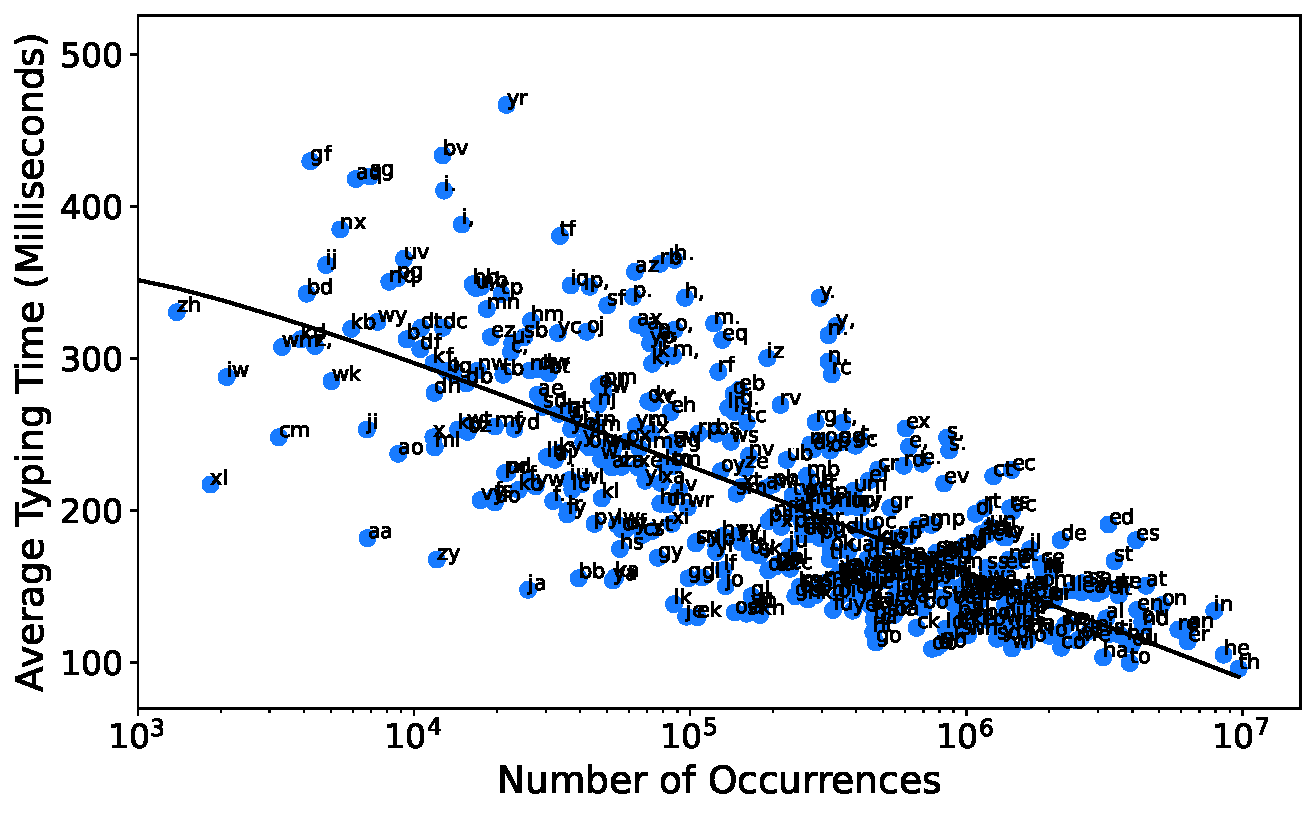
\includegraphics[width=\columnwidth]{figures/freqplot.pdf}
\caption{Relationship Between English Bigram Frequency and Average Typing Time on QWERTY}
\label{fig:freq_to_time}
\end{figure}

\begin{figure}[h]
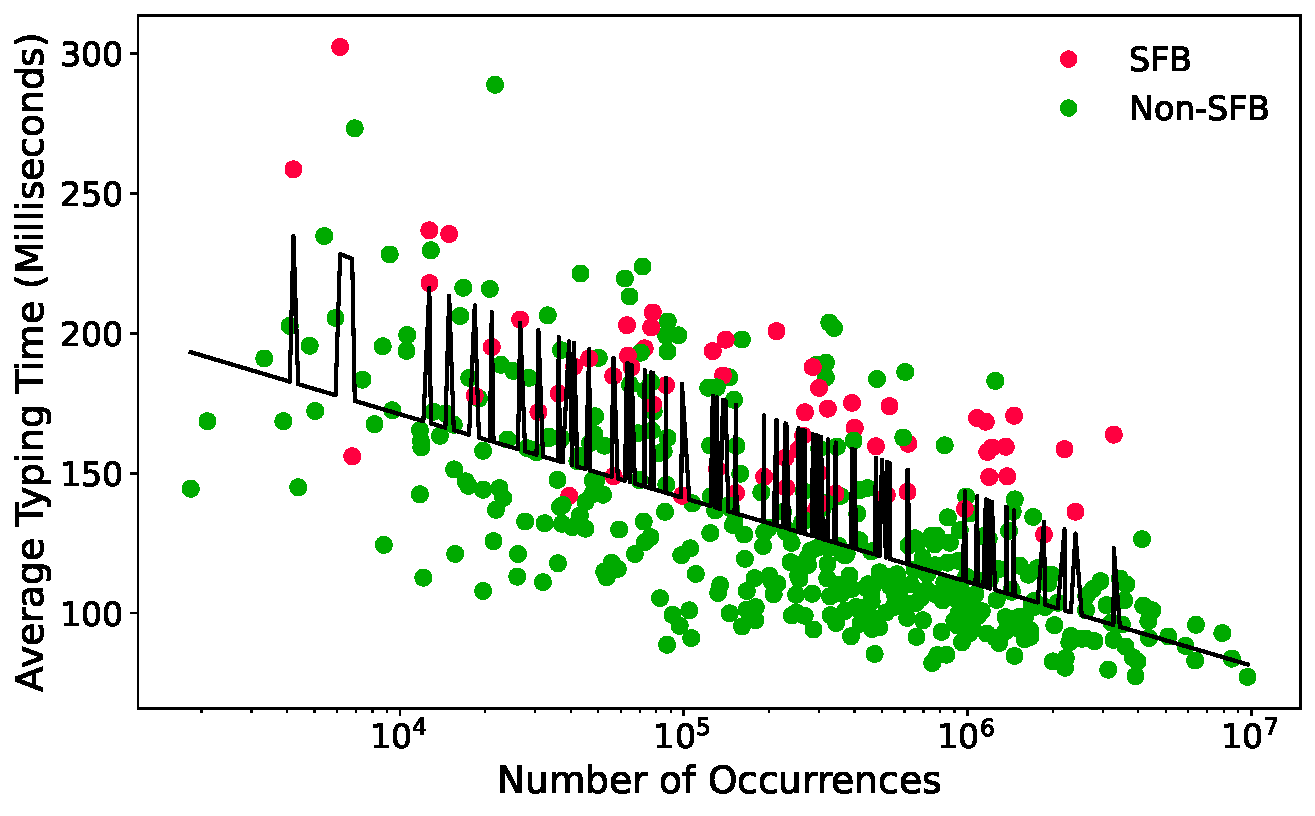
\includegraphics[width=\columnwidth]{figures/sfbplot.pdf}
\caption{The Effect of SFBs and Frequency on Typing Time ($>80$WPM)}
\label{fig:bigram_typing_time}
\end{figure}

\subsubsection{Tristroke Analysis}
\noindent Several features unique to tristrokes were identified; however, they were excluded from the analysis due to their low statistical significance  and the increased risk of overfitting the model. The only exception to this exclusion is the single-finger skipstroke category. Single-finger skipstrokes, like single-finger bistrokes, involve two strokes made by the same finger, but with an intervening stroke between them. An example of this on the QWERTY keyboard is the word "fit," as both the 'f' and 't' are typed with the left index finger, leading to a coordinative delay. Single-finger skipstrokes are important to consider because, for fast typists, they function similarly to single-finger bistrokes with an added delay. Since single-finger bistrokes notably impact typing speed -- especially at higher typing speeds -- accounting for single-finger skipstrokes is imperative when targeting faster typing speeds.



 %  and may be important for different models
% Tristroke analysis merits future exploration.
% Time prediction for tristrokes is performed by taking the sum of the tristroke's constituent bistrokes and adding a small as they make up most of the time fluctuations associated with a given tristroke.
\subsection{Creating the Objective Function}
The objective function we are optimizing for is the predicted time to type a corpus on a specific layout in a given WPM range. This prediction is achieved by evaluating the cost, or typing time, of each trigram within the corpus, multiplying it by the trigram's occurrence count, and summing the results, yielding the estimated time required to type the corpus on that particular layout.

The limited diversity of layouts in the dataset makes developing an accurate time prediction model challenging, as it has the potential to introduce significant bias. The averaging of typing times further reduces the effective sample size, amplifying the risk of overfitting to the specific nuances of these layouts. To mitigate this risk, a cost function is devised based on insights from our data analysis, and the number of adjustable parameters within the cost function is minimized. The adjustable parameters are later fine-tuned using the Levenberg-Marquardt algorithm. This approach, in contrast to more complex techniques such as neural networks, helps prevent overfitting by retaining only the most salient relationships observed in the data. 

% to enhance the model's efficacy for layouts not present in the training data

% Calculation of the tristroke cost function relies on a bistroke cost function. 

Calculation of the tristroke cost function relies on first calculating the cost of its constituent bistrokes. So we first define the bistroke cost function, $C(b)$, as the predicted time required to type a given bistroke $b$ of category $i$, with base positional penalties $P_x$ and $P_y$, categorical positional penalties $P^{(i)}_x$ and $P^{(i)}_y$, and a frequency penalty $f(b)$. The frequency penalty is modeled using a logarithmic function with free parameters $p_1$, $p_2$, and $p_3$. The columnar penalties, $P_x$ and $P^{(i)}_x$, are calculated based on the absolute value of the x-coordinate for the second keystroke in the bistroke. Taking the absolute value is done to limit any potential hand bias that could stem from adaptive behaviors to an uneven workload. A free parameter is assigned to each possible column value to weight its influence on typing speed. % = \{ 1,2,3 \}

The row penalties, $P_y$ and $P^{(i)}_y$, are calculated based on the y-coordinate of the second key in the bistroke. Each possible y-coordinate is assigned a free parameter to weight its effect on typing speed. It is assumed that a row-staggered keyboard is used, as it is the most common layout. On a row-staggered keyboard, the top row has a $-0.25$ key offset, and the bottom row has a $0.5$ key offset. This offset must be accounted for in the single-finger bistroke's distance calculation, so $\Delta$ is introduced to represent the row-stagger-adjusted distance between keys. For any other bistroke, $\Delta$ is set to $0$. A free parameter, $p_4$, is added to $\Delta$ to establish a baseline penalty weight. This parameter determines the extent to which distance contributes to the penalty on top of the row-stagger adjustment and also prevents $\Delta$ from becoming zero, which would negate the placement penalties. The bistroke cost function, $C(b)$, is calculated as the product of the finger penalties and the frequency logarithm.
\begin{equation*}
    \begin{split}
        C(b) &= \left(p_1 \log (f(b) + p_2) + p_3\right) \\
             &\quad \times \left(1 + P_x(b) P_y(b) + P^{(i)}_x(b) P^{(i)}_y(b) (\Delta + p_4) \right)  
    \end{split}
\end{equation*}

\noindent For the tristroke cost function $C(t)$, we take the sum of the cost of its constituent bistrokes $b_1(t)$ and $b_2(t)$, then add a small penalty for the trigram's associated skipstroke $s(t)$, if it is a single-finger skipstroke. The single-finger skipstroke penalty, like the single-finger bistroke penalty, considers positional penalties $P_x$ and $P_y$, as well as a distance penalty $(\Delta + p_5)$ with a free parameter $p_5$. It should be noted that the single-finger skipstroke penalty defaults to $0$ if there is no single-finger skipstroke.  %, which defaults to $0$ if the trigram is not a single-finger skipstroke.
\begin{equation*}
C(t) = C(b_1(t)) + C(b_2(t)) + P_x(s(t))  P_y(s(t)) (\Delta + p_5)
\end{equation*}

\noindent Finally, the data is limited to the desired WPM range. The bistroke cost function is then fit to the bistroke data, and the tristroke cost function is fit to the tristroke data, using the Levenberg-Marquardt algorithm. The MAE of the fit changes depending on the target WPM, but the $R^2$ metric remains constant. For $80$ WPM, this results in $C(b)$ having an MAE of $12$ milliseconds and an $R^2$ of $0.78$. $C(t)$ is less accurate with an MAE of $26$ milliseconds and an $R^2$ of $0.42$. The cumulative cost $C(l)$ for a layout $l$ is the sum of each tristroke's predicted typing time multiplied by its number of occurrences, effectively estimating the typing time for a given layout across the corpus.
\begin{equation*}
C(l) = \sum_{t \in T} (C(t) \times f(t) )
\end{equation*}

\noindent This is the objective function passed onto the simulated annealing algorithm for optimization.

%which is what the simulated annealing algorithm optimizes for, is 



\subsection{Simulated Annealing}


\textit{Simulated annealing} is a metaheuristic optimization technique inspired by the annealing process in metallurgy, where metals are cooled gradually to achieve a stable state with minimized energy \citep{kirkpatrick1983optimization}. In the context of keyboard optimization, it is used as an iterative algorithm that explores different keyboard layouts by gradually accepting key swaps that reduce the overall energy (i.e., predicted typing time). Unlike gradient descent and other methods that always aim for an absolute minimum, simulated annealing allows for the occasional acceptance of higher-cost solutions to explore a broader search space, preventing the algorithm from getting stuck in local optima. Eventually, simulated annealing converges toward a stable, low-cost configuration -- the global minimum or an approximation of it. 

% A key challenge in applying simulated annealing effectively lies in selecting appropriate parameters that govern the algorithm's behavior, including the initial temperature and the termination criterion. These parameters can significantly influence the algorithm's convergence and the quality of the solution obtained. Traditionally, parameter selection has relied on manual estimation based on domain knowledge and experimentation, which can be time-consuming and may not generalize well across different problem instances \citep{Ben-Ameur2004}. To address this, this paper outlines a dynamic approach to setting the initial temperature and termination criterion, allowing for greater flexibility and adaptability when exploring layouts under various data modifications. For example, analyzing layouts at different WPM ranges, optimizing for specific subsets of keys, or using different corpora can lead to substantial variations in the cost function and the number of swaps required for convergence. The dynamic parameter setting approach ensures that the simulated annealing algorithm can effectively explore the solution space and converge towards an optimal layout, regardless of these variations.


Selecting the parameters in simulated annealing for convergence can be challenging, usually requiring experimentation or domain knowledge \citep{SAOverview}. We outline a dynamic approach to setting the initial temperature and termination criterion to address this. This ensures layouts can be explored across a variety of data modifications. For example, layouts may be optimized for different WPM ranges, languages, or a specific subset of keys. In these cases, the cost function may yield drastically different values, and the number of swaps required for convergence may vary, necessitating adjustments to the parameters.

% Proofs of the simulated annealing's effectiveness are outside of the scope of this paper.
\subsubsection{Solution Space and Transitions}
\noindent A crucial step in implementing simulated annealing is defining the solution space and transition process. This allows the algorithm to explore potential solutions effectively. Changes to the solution should occur gradually to ensure smooth traversal of the solution landscape, preventing abrupt jumps that overlook promising solutions \citep{SAOverview}.

For keyboard optimization, a solution is defined as a mapping between characters and their positions on a matrix, as illustrated in Table ~\ref{fig:keyboard_matrix}. The chosen coordinate system mirrors real-world keyboard usage by grouping fingers based on absolute values, differentiating hands by sign, and enabling easy distance calculations. This encoding strategy allows the algorithm to effectively evaluate the ergonomic implications of different key arrangements. A transition is defined as the swapping of two keys on the keyboard matrix. % Consequently, the neighborhood of a given layout consists of all layouts that can be generated as the result of a single key pair swap.

The acceptance of candidate solutions in simulated annealing is determined by a probabilistic criterion derived from the Boltzmann distribution function. Originating from statistical mechanics, this function describes the probability of particles occupying different energy states within a system \citep{harris2004introduction}. This criterion is mathematically represented as follows:

\begin{equation*}
A(i) = 
\left\{ 
\begin{array}{lr}
    \exp \left( -\frac{\Delta E}{T} \right), & \text{if } \Delta E > 0 \\
    1, & \text{otherwise}
\end{array}
\right.
\end{equation*}

\noindent Here, $\Delta E$ represents the change in energy within the system or, in this case, in the estimated typing time between the current layout and the candidate layout, and $T$ denotes the temperature, a parameter that controls the amount of randomness in the system. If the change in typing time is negative ($\Delta E < 0$), indicating an improvement in estimated typing time, the candidate layout is accepted with certainty. However, if the change in estimated typing time is positive, indicating a worsening layout, the candidate layout is accepted with a probability determined by the Boltzmann factor, which is more likely to accept slight decreases in performance over larger ones.

This choice of probabilistic criterion allows the simulated annealing algorithm to converge on an optimal or near-optimal solution through gradual refinement \citep{granville1994simulated}. Initially, the temperature is high, allowing the algorithm to explore the solution space and escape local minima by accepting suboptimal moves. As the algorithm progresses and the temperature decreases, the probability of accepting suboptimal moves diminishes, refining the search to more promising regions. The reduction in temperature is controlled by a cooling schedule, which dictates how fast and effectively the algorithm converges to a solution. We adopt a monotonically decreasing geometric cooling schedule defined as follows:
\begin{equation*}
T_i = \alpha^i T_0
\end{equation*}

\noindent where $T_0$ is the initial-temperature and $a$ is the cooling-rate, $0 < a < 1$.

\begin{figure}[h]
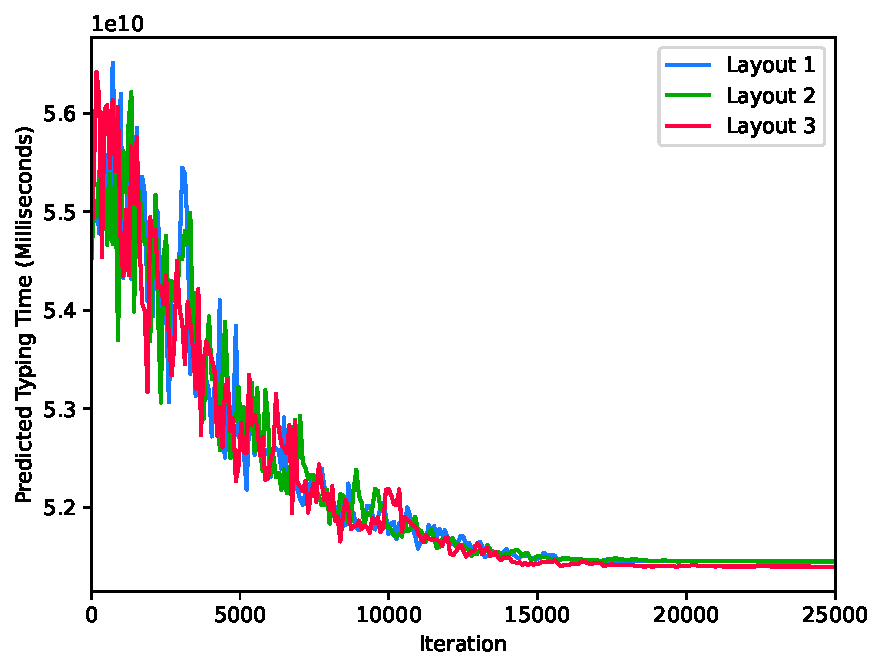
\includegraphics[width=\columnwidth]{figures/convergence.pdf}
\caption{Convergence of Estimated Typing Time during Simulated Annealing}
\label{fig:bigram_typing_time}
\end{figure}



\subsubsection{Setting the Initial Temperature}
\noindent Before any transitions are performed, an initial temperature must be set for the cooling schedule to iterate on. A common approach to setting the initial temperature is to manually estimate it based on the problem domain and its characteristics. This initial temperature is frequently chosen so that the acceptance probability at the beginning of simulated annealing is approximately equal to some value. Lacking relevant literature for our problem domain, we resort to the approach outlined in  ~\citet{Ben-Ameur2004}. We set a variable $\chi_0$ to be the desired initial acceptance probability of suboptimal transitions at the beginning of the algorithm. An iterative method is employed to compute the initial temperature $T_0$ such that the acceptance probability approaches $\chi_0$. To compute the estimated acceptance probability $\hat{\chi}(T)$ for a given temperature $T$, first, we use the set $S$ of possible positive transitions (i.e., transitions where $E_{before} < E_{after}$), where each transition $s$ represents a swap of two keys. Finally, we take the ratio between the sum of probabilities of generating and accepting each positive transition $s$ and the sum of the probabilities of generating each positive transition $s$:
\begin{equation*}
\hat{\chi}(T_n) = \frac{
    \sum_{s \in S} \exp \left( -\frac{E_{after}(s)}{T_n} \right)}
    {\sum_{s \in S} \exp \left( -\frac{E_{before}(s)}{T_n} \right)}
\end{equation*}
This can now be used to find $T_0$. First, we define an initial guess temperature $T_1$, then recursively apply this formula:
\begin{equation*}
T_{n+1} = T_n \left(\frac{\ln(\hat{\chi}(T_n))}{\ln{(\chi_0)}} \right)
\end{equation*}
Once $|\hat{\chi}(T_n) - \chi_0| \leq \epsilon$ for some error $\epsilon$, we have found our initial temperature $T_0$. 

\subsubsection{Termination Criterion}
\noindent Finally, we establish a termination criterion for the simulated annealing process to be the point at which the number of iterations lacking improvement reaches the probabilistic threshold that all potential swaps have been evaluated. We do this to ensure the simulated annealing algorithm has settled on some minima while allowing suboptimal swaps to be heuristically accepted, potentially escaping local minima.

To find the termination criterion, let $S$ be the number of iterations to evaluate all potential swaps. Let $k$ be the number of keys; for $k$ keys, the number of swappable key pairs $n = \binom{k}{2}$. We consider $S = \sum_{i=1}^{n} s_i$ where $s_i$ is the number of iterations required to evaluate the $i$-th pair after $i-1$ pairs have been evaluated.

The probability $P_i$ of selecting a new pair to swap is $P_i = \frac{n-(i-1)}{n} = \frac{n-i+1}{n}$. Consequently, $s_i$ follows a geometric distribution with an expectation of $\text{E}(s_i) = \frac{n}{n-i+1}$.

\noindent By the linearity of expectations, we derive:
\begin{align*}
\text{E}(S) = n \sum_{i=1}^{n} \frac{1}{i}
\end{align*}
To increase performance, we can use the approximation:
\begin{align*}
\text{E}(S) = n \log{n} + \gamma n + \frac{1}{2} +  O\left(\frac{1}{n}\right)
\end{align*}
where $\gamma \approx 0.5772156649$ is the Euler-Mascheroni constant. Since the number of iterations must be a positive integer, we set our final stopping point to be:
\begin{align*}
\left\lceil \binom{k}{2} \log{\binom{k}{2}} + \gamma \binom{k}{2} + \frac{1}{2} \right\rceil
\end{align*}


% \noindent The layout produced in this paper optimizes for the main block of 30 keys. So the number of possible swaps is $\binom{30}{2} = 435$ resulting in a stopping point of $\left\lceil \binom{30}{2} \log{\binom{30}{2}} + \gamma \binom{30}{2} + \frac{1}{2} \right\rceil = 2,895$ iterations.

% Manual newpage inserted to improve layout of sample file - not
% needed in general before appendices/bibliography.
\section{Results}

For the final layout, we choose to use the 30 most common characters in our corpus, which is the standard English alphabet, plus the addition of four special characters: the comma, period, hyphen, and apostrophe. This layout differs by 2 characters from the QWERTY layout, so to compare the final layout with QWERTY requires we only predict the time for strings in the corpus that can be typed on both layouts. Although the average typing speed was $47$ WPM, we set the target WPM to $\geq80$ as a litmus test of proficiency. This results in single-finger bistrokes having greater impact and frequency having less. Optimizing for an above-average WPM like this is desirable if the goal is to raise the upper threshold of potential typing speed. Using the methodology in this paper, one could also aim to optimize for the average user, improving the mean speed. The resulting layout can be seen in Table \ref{fig:keyboard1}.
\begin{table}[h]
\caption{Generated Layout for Typing Speeds $\geq80$ WPM}
\begin{center}
\tiny
\renewcommand{\arraystretch}{1.5}
\begin{tabularx}{\columnwidth}{ | *{10}{>{\centering\arraybackslash}X|} }
\hline
\textbf{M} & \textbf{R} & \textbf{T} & \textbf{C} & \textbf{W} & \textbf{,} & \textbf{K} & \textbf{A} & \textbf{E} & \textbf{'} \\ \hline
\textbf{L} & \textbf{N} & \textbf{D} & \textbf{S} & \textbf{V} & \textbf{Y} & \textbf{U} & \textbf{O} & \textbf{I} & \textbf{G} \\ \hline
\textbf{H} & \textbf{X} & \textbf{Z} & \textbf{B} & \textbf{F} & \textbf{.} & \textbf{-} & \textbf{Q} & \textbf{J} & \textbf{P} \\ \hline
\multicolumn{10}{|c|}{\multirow{1}{*}{\textbf{SPACE}}} \\ \hline
\end{tabularx}
\end{center}
\label{fig:keyboard1}
\end{table}




\noindent The predicted time to type the iWeb corpus on QWERTY is 54,934,582 seconds, Dvorak is 52,565,249 seconds, a speed up of $~4\%$, and the layout produced in this paper is predicted to take 51,429,827 seconds, a speed up of $~6\%$. Our analysis revealed positional categories of bistroke that played a significant role in the prediction of typing speed. Namely, ALTs which are shown to be faster and SFBs which are shown to be slower. For QWERTY, $18.3\%$ of all bistrokes are ALTs and $5.7\%$ of them are SFBs, dvorak has $33.6\%$ ALTs and $2.8\%$ SFBs, and the layout produced in this paper has the best result of $33.6\%$ ALTs and $1.4\%$ SFBs. The fact that speed optimization yields only marginal improvements in typing efficiency is not unexpected but remains a valuable take away, as it suggests prioritizing theoretical features over solely focusing on speed optimization may offer substantial benefits.

% colemak and dvorak here

\section{Future Work}
The overrepresentation of the QWERTY, AZERTY, and QWERTZ layouts in the current data set likely biases the model, as evidenced by the observed preference for the top row. The sparsity of data may impair the model's ability to generalize accurately. Although the proposed cost function is simple and generalizable, it does not fully capture the complexities of human typing behavior. Future studies should prioritize the collection of data from a wider variety of keyboard layouts and typing speeds to mitigate this limitation. To facilitate this, an open-source tool, Kiakl, was developed to crowdsource data from alternative keyboard layouts. However, due to time constraints and the limited volume of data gathered, Kiakl was not used in this study. A more comprehensive data set would enable the exploration of more sophisticated models, such as transformers or recurrent neural networks, offering the potential for a more nuanced and accurate evaluation of keyboard layouts.

The incorporation of previously excluded tristroke and bistroke features also warrants consideration. These features include lateral stretches, redirects, rolls, and scissors. A lateral stretch occurs when two adjacent fingers are pulled apart horizontally, complicating the articulation of a bistroke. These occur almost exclusively from keystrokes in the inner index columns. Scissors occur when one finger of a hand reaches towards the top row, while another finger on the same hand contracts to press a key on the bottom row. Redirects occur when a tristroke, typed with the same hand, changes direction, frequently resulting in typos. An example of this in the QWERTY layout is the tristroke "sad," as the "sa" is typed outward while "ad" is typed inward. A roll occurs when a tristroke is typed with the same hand and maintains a consistent direction, which may be faster to articulate. Modeling these movements may increase predictive accuracy, offering opportunities for further optimization. 
% These movements, though subtle and nuanced, represent important articulation dynamics that can influence typing speed and efficiency, offering opportunities optimization.

Further improvements to the keyboard optimization process could involve refining the simulated annealing algorithm itself. Although geometric cooling was effective in this study, exploring alternative cooling schedules could improve performance. Modifying the cooling rate over time or experimenting with alternative patterns, such as polynomial or logarithmic decays, may enhance the algorithm's ability to find global optima. Finally, incorporating formal mathematical validation, such as estimating the lower bound of optimization, would help verify and guide future results.
% left hand right hand
% Integrating other metaheuristic algorithms, like genetic algorithms or particle swarm optimization, could provide valuable insights and alternative approaches for optimization.

% more data, kiakl, looking for ways of measuring comfort that are valid


%% The next two lines define the bibliography style to be used, and
%% the bibliography file.
\balance
\bibliographystyle{ACM-Reference-Format}
\bibliography{sample-base}

\end{document}
\endinput
%%
%% End of file `sample-sigplan.tex'.